\documentclass{beamer}
\usepackage[utf8]{inputenc}

\usetheme{Madrid}
\usecolortheme{default}
\usepackage{amsmath,amssymb,amsfonts,amsthm}
\usepackage{mathtools}
\usepackage{txfonts}
\usepackage{tkz-euclide}
\usepackage{listings}
\usepackage{adjustbox}
\usepackage{tfrupee}
\usepackage{array}
\usepackage{gensymb}
\usepackage{tabularx}
\usepackage{gvv}
\usepackage{lmodern}
\usepackage{circuitikz}
\usepackage{tikz}
\lstset{literate={·}{{$\cdot$}}1 {λ}{{$\lambda$}}1 {→}{{$\to$}}1}
\usepackage{graphicx}

\setbeamertemplate{page number in head/foot}[totalframenumber]

\usepackage{tcolorbox}
\tcbuselibrary{minted,breakable,xparse,skins}

\definecolor{bg}{gray}{0.95}
\DeclareTCBListing{mintedbox}{O{}m!O{}}{%
  breakable=true,
  listing engine=minted,
  listing only,
  minted language=#2,
  minted style=default,
  minted options={%
    linenos,
    gobble=0,
    breaklines=true,
    breakafter=,,
    fontsize=\small,
    numbersep=8pt,
    #1},
  boxsep=0pt,
  left skip=0pt,
  right skip=0pt,
  left=25pt,
  right=0pt,
  top=3pt,
  bottom=3pt,
  arc=5pt,
  leftrule=0pt,
  rightrule=0pt,
  bottomrule=2pt,
  toprule=2pt,
  colback=bg,
  colframe=orange!70,
  enhanced,
  overlay={%
    \begin{tcbclipinterior}
    \fill[orange!20!white] (frame.south west) rectangle ([xshift=20pt]frame.north west);
    \end{tcbclipinterior}},
  #3,
}
\lstset{
    language=C,
    basicstyle=\ttfamily\small,
    keywordstyle=\color{blue},
    stringstyle=\color{orange},
    commentstyle=\color{green!60!black},
    numbers=left,
    numberstyle=\tiny\color{gray},
    breaklines=true,
    showstringspaces=false,
}

\title{12.755}
\date{October 10, 2025}
\author{Bhargav - EE25BTECH11013}

\begin{document}

\frame{\titlepage}

\begin{frame}{Question}
\textbf{Question}: \\
Which one of the following vectors is an eigenvector corresponding to the eigenvalue $\lambda = 1$ for the matrix 
\begin{align}
\vec{A} = \myvec{1 & 1 & 0 \\  1 & -1 & 0 \\ 1 & -1 & 1}
\end{align}
is
\end{frame}

\begin{frame}{Solution}
The eigenvalue of the the the matrix $\vec{A}$ can be found out by (where $\lambda=1$ is the eigenvalue, $\vec{x}$ is the eigenvector, $\vec{I}$ is the identity matrix)

\begin{align}
\vec{A}\vec{x} = \lambda \vec{x} \implies \vec{A}\vec{x} = \vec{x}
\end{align}
\begin{align}
\brak{\vec{A}-\vec{I}}\vec{x} = \vec{0}
\end{align}
\begin{align}
\implies \myvec{0 & 1 & 0 \\ 1 & -2 & 0 \\ 1 & -1 & 0}\vec{x} = \vec{0}
\end{align}
\end{frame}

\begin{frame}{Solution}
This can be solved by representing it as an augmented matrix and using row elimination
\begin{align}
\augvec{3}{1}{
0 & 1 & 0 & 0 \\
1 & -2 & 0 & 0 \\
1 & -1 & 0 & 0
}
\xleftrightarrow{R_1 \leftrightarrow R_2}
\augvec{3}{1}{
1 & -2 & 0 & 0 \\
0 & 1 & 0 & 0 \\
1 & -1 & 0 & 0
}
\xleftrightarrow{R_3 \leftarrow R_3 - R_1}
\end{align}
\begin{align}
\augvec{3}{1}{
1 & -2 & 0 & 0 \\
0 & 1 & 0 & 0 \\
0 & 1 & 0 & 0
}
\xleftrightarrow{R_3 \leftarrow R_3 - R_2}
\augvec{3}{1}{
1 & -2 & 0 & 0 \\
0 & 1 & 0 & 0 \\
0 & 0 & 0 & 0
}
\end{align}
\end{frame}

\begin{frame}{Solution}
Thus $\vec{x} = t\myvec{0 \\ 0 \\ 1}$ where $t \in \mathbf{R}$ \\
So, the eigenvector of $\vec{A}$ is $\myvec{0 \\ 0 \\ 1}$ \\ \\ \\

This can be further verified by the intersection of planes
\begin{align}
x - 2y = 0
\end{align}
\begin{align}
y = 0
\end{align}
\end{frame}
\begin{frame}{Plot}
    \begin{figure}[H]
        \centering
        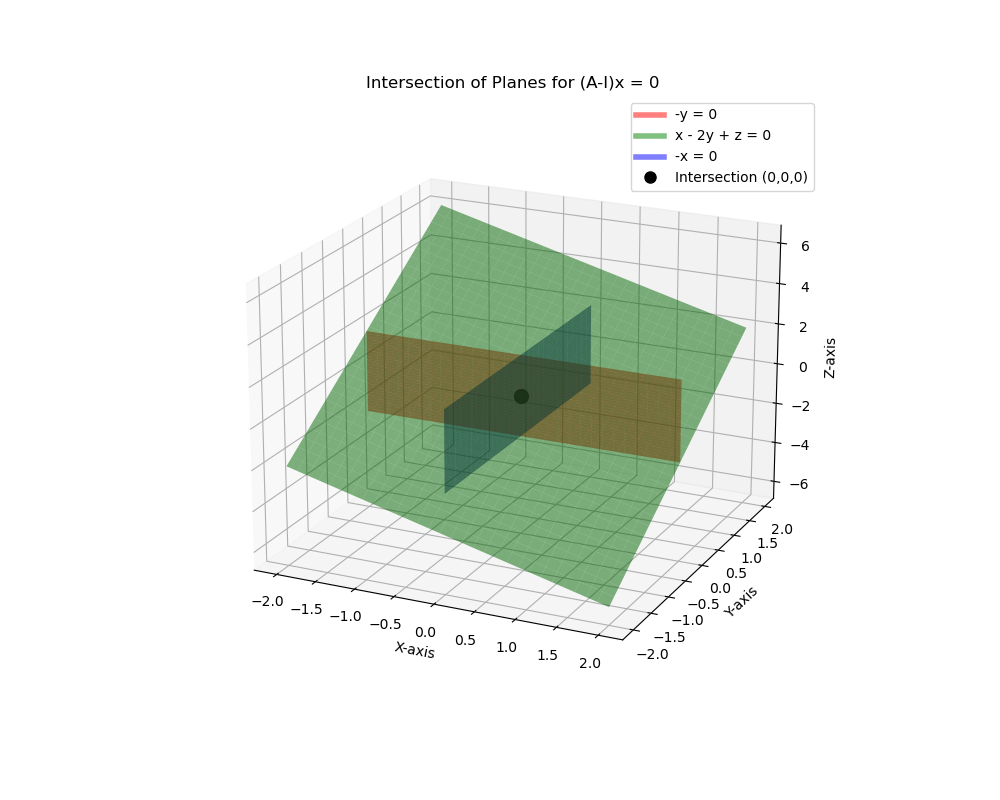
\includegraphics[height=0.5\textheight, keepaspectratio]{figs/Figure_1.png}
    \end{figure}
\end{frame}
\begin{frame}[fragile]
    \frametitle{C Code}
    \begin{lstlisting}
#include <stdio.h>
#include <stdlib.h>

void generate_plane1(double *Y, double *Z, double *X, int N) {
    for(int i = 0; i < N*N; i++) {
        X[i] = 2 * Y[i];
    }
}

void generate_plane2(double *X, double *Z, double *Y, int N) {
    for(int i = 0; i < N*N; i++) {
        Y[i] = 0;
    }
}


    \end{lstlisting}
\end{frame}
\begin{frame}[fragile]
    \frametitle{C Code}
    \begin{lstlisting}

void generate_intersection_line(double *x, double *y, double *z, int N) {
    double dz = 4.0/(N-1);
    for(int i = 0; i < N; i++) {
        x[i] = 0;
        y[i] = 0;
        z[i] = -2 + i*dz;
    }
}



    \end{lstlisting}
\end{frame}

\begin{frame}[fragile]
    \frametitle{Python + C Code}
    \begin{lstlisting}
import numpy as np
import ctypes
import matplotlib.pyplot as plt
from matplotlib.lines import Line2D

lib = ctypes.CDLL("./libplanes.so")

N = 40
d = np.linspace(-2, 2, N)
Y, Z = np.meshgrid(d, d)
X = np.zeros_like(Y)




    \end{lstlisting}
\end{frame}
\begin{frame}[fragile]
    \frametitle{Python + C Code}
    \begin{lstlisting}
# Convert to C-contiguous arrays
Y_c = np.ascontiguousarray(Y, dtype=np.double)
Z_c = np.ascontiguousarray(Z, dtype=np.double)
X_c = np.ascontiguousarray(X, dtype=np.double)

# Set argument types
lib.generate_plane1.argtypes = [np.ctypeslib.ndpointer(dtype=np.double),
                                np.ctypeslib.ndpointer(dtype=np.double),
                                np.ctypeslib.ndpointer(dtype=np.double),
                                ctypes.c_int]

lib.generate_plane2.argtypes = [np.ctypeslib.ndpointer(dtype=np.double),
                                np.ctypeslib.ndpointer(dtype=np.double),
                                np.ctypeslib.ndpointer(dtype=np.double),
                                ctypes.c_int]

lib.generate_intersection_line.argtypes = [np.ctypeslib.ndpointer(dtype=np.double, ndim=1, flags='C_CONTIGUOUS'),
                                           np.ctypeslib.ndpointer(dtype=np.double, ndim=1, flags='C_CONTIGUOUS'),
                                           np.ctypeslib.ndpointer(dtype=np.double, ndim=1, flags='C_CONTIGUOUS'),
                                           ctypes.c_int]




    \end{lstlisting}
\end{frame}
\begin{frame}[fragile]
    \frametitle{Python + C Code}
    \begin{lstlisting}
# Generate plane1
lib.generate_plane1(Y_c, Z_c, X_c, N)

# Plotting
fig = plt.figure(figsize=(10, 8))
ax = fig.add_subplot(111, projection='3d')

ax.plot_surface(X_c, Y_c, Z_c, alpha=0.5, color='g')

# Plane 2
X2, Z2 = np.meshgrid(d, d)
Y2 = np.zeros_like(X2)
lib.generate_plane2(X2, Z2, Y2, N)
ax.plot_surface(X2, Y2, Z2, alpha=0.5, color='r')

# Intersection line
x_line = np.zeros(N)
y_line = np.zeros(N)

    \end{lstlisting}
\end{frame}

\begin{frame}[fragile]
    \frametitle{Python + C Code}
    \begin{lstlisting}
z_line = np.zeros(N)
lib.generate_intersection_line(x_line, y_line, z_line, N)
ax.plot3D(x_line, y_line, z_line, color='k', linewidth=3)

# Intersection point at origin
ax.scatter(0,0,0,color='black',s=80)

# Legend
legend_elements = [
    Line2D([0],[0], color='g', lw=4, alpha=0.5, label='x - 2y = 0'),
    Line2D([0],[0], color='r', lw=4, alpha=0.5, label='y = 0'),
    Line2D([0],[0], color='k', lw=3, label='Intersection Line (x=0, y=0)'),
    Line2D([0],[0], marker='o', color='k', label='Origin (0,0,0)', markersize=8, linestyle='')
]
ax.legend(handles=legend_elements)

ax.set_xlabel('X-axis'); ax.set_ylabel('Y-axis'); ax.set_zlabel('Z-axis')
ax.set_title('Intersection of Planes: x - 2y = 0 and y = 0')
ax.view_init(elev=25, azim=-60)

plt.savefig("/mnt/c/Users/bharg/Documents/backupmatrix/ee25btech11013/matgeo/12.755/figs/Figure_1.png")

plt.show()
    \end{lstlisting}
\end{frame}
\begin{frame}[fragile]
    \frametitle{Python Code}
    \begin{lstlisting}
import numpy as np
import matplotlib.pyplot as plt
from matplotlib.lines import Line2D

fig = plt.figure(figsize=(10, 8))
ax = fig.add_subplot(111, projection='3d')

d = np.linspace(-2, 2, 40)
Y, Z = np.meshgrid(d, d)  # create grid

# Plane 1: x - 2y = 0 → X = 2Y, Z free
X1 = 2 * Y
Z1 = Z
ax.plot_surface(X1, Y, Z1, alpha=0.5, color='g')

# Plane 2: y = 0 → Y=0, X and Z free
X2, Z2 = np.meshgrid(d, d)
Y2 = np.zeros_like(X2)
ax.plot_surface(X2, Y2, Z2, alpha=0.5, color='r')



    \end{lstlisting}
\end{frame}
\begin{frame}[fragile]
    \frametitle{Python Code}
    \begin{lstlisting}
# Intersection line: x=0, y=0, z free
z_line = np.linspace(-2, 2, 20)
x_line = np.zeros_like(z_line)
y_line = np.zeros_like(z_line)
ax.plot3D(x_line, y_line, z_line, color='k', linewidth=3)

# Intersection point at origin
ax.scatter(0, 0, 0, color='black', s=80)

    \end{lstlisting}
\end{frame}
\begin{frame}[fragile]
    \frametitle{Python Code}
    \begin{lstlisting}

# Legend
legend_elements = [
    Line2D([0],[0], color='g', lw=4, alpha=0.5, label='x - 2y = 0'),
    Line2D([0],[0], color='r', lw=4, alpha=0.5, label='y = 0'),
    Line2D([0],[0], color='k', lw=3, label='Intersection Line (x=0, y=0)'),
    Line2D([0],[0], marker='o', color='k', label='Origin (0,0,0)', markersize=8, linestyle='')
]
ax.legend(handles=legend_elements)

ax.set_xlabel('X-axis')
ax.set_ylabel('Y-axis')
ax.set_zlabel('Z-axis')
ax.set_title('Intersection of Planes: x - 2y = 0 and y = 0')
ax.view_init(elev=25, azim=-60)
plt.savefig("/mnt/c/Users/bharg/Documents/backupmatrix/ee25btech11013/matgeo/12.755/figs/Figure_1.png")

plt.show()



    \end{lstlisting}
\end{frame}


\end{document}
